\section{Модель сухого электронно-лучевого травления резиста} \label{sec:DEBER_model}

Объединение моделей рассеяния электронного пучка, электронно-стимулированных разрывов молекул ПММА, электронно-стимулированной термической деполимеризации ПММА, диффузии мономера и растекания ПММА позволило создать модель процесса СЭЛТР. На ее основе был разработан алгоритм моделирования профиля линии, получаемой методом СЭЛТР при произвольных параметрах процесса. В данном алгоритме все время экспонирования разделялось на промежутки величиной 1~с, и на каждом промежутке последовательно выполнялись следующие действия:

\begin{enumerate}
	\item Моделирование рассеяния электронного пучка в системе ПММА/Si;
	\item Моделирование электронно-стимулированных разрывов молекул \linebreak ПММА;
	\item Моделирование электронно-стимулированной термической деполимеризации ПММА;
	\item Определение подвижностей вершин поверхности слоя ПММА;
	\item Вычисление положений и объемов микрополостей в слое ПММА;
	\item Преобразование слоя ПММА со внутренними микрополостями в сплошную пилообразную структуру;
	\item Моделирование растекания пилообразной структуры;
	\item Определение нового положения поверхности слоя ПММА.
\end{enumerate}
По истечении времени экспонирования моделировалось растекание слоя ПММА при охлаждении образца до температуры, при которой процессы растекания переставали протекать заметным образом (было установлено, что эта температура составляет около 80~$^{\circ}$C).

Демонстрация процесса моделирования профиля линии, получаемой методом СЭЛТР, приведена на рисунке~\ref{fig:DEBER_example}.
Моделирование проводилось для следующих условий условий экспонирования: начальная толщина слоя ПММА равна 500~нм, энергия электронного пучка $E$ = 20 кэВ, температура образца $T$~=~150~$^{\circ}$C/c, время экспонирования $t_\mathrm{exp}$ = 100 с, плотность тока экспонирования на единицу длины $j_\mathrm{l}$ = 10 пА/см.
Распределение плотности тока в пучке считалось нормальным со среднеквадратичным отклонением, равным 300 нм.
Скорость охлаждения образца после экспонирования составляла 1~$^{\circ}$C/с.

\begin{figure}[h!]
	\begin{minipage}{0.48\textwidth}
%		\includegraphics[width=\linewidth]{DEBER_example/example_20_200} \\
		\includegraphics[width=\linewidth]{DEBER_example/example_15_NEW_2} \\
		\vspace{-13em} \\ \text{\hspace{0em} a}) \\ \vspace{13em}
	\end{minipage}
	\begin{minipage}{0.48\textwidth}
%		\includegraphics[width=\linewidth]{DEBER_example/example_70_200} \\
		\includegraphics[width=\linewidth]{DEBER_example/example_65_NEW_2} \\
		\vspace{-13em} \\ \text{\hspace{-0.1em} б}) \\ \vspace{13em}
	\end{minipage}
	
	\vspace{-3em}
	
	\begin{minipage}{0.48\textwidth}
%		\includegraphics[width=\linewidth]{DEBER_example/example_99_200} \\
		\includegraphics[width=\linewidth]{DEBER_example/example_99_NEW_2} \\
		\vspace{-13em} \\ \text{\hspace{0em} в}) \\ \vspace{13em}
	\end{minipage}
	\begin{minipage}{0.48\textwidth}
%		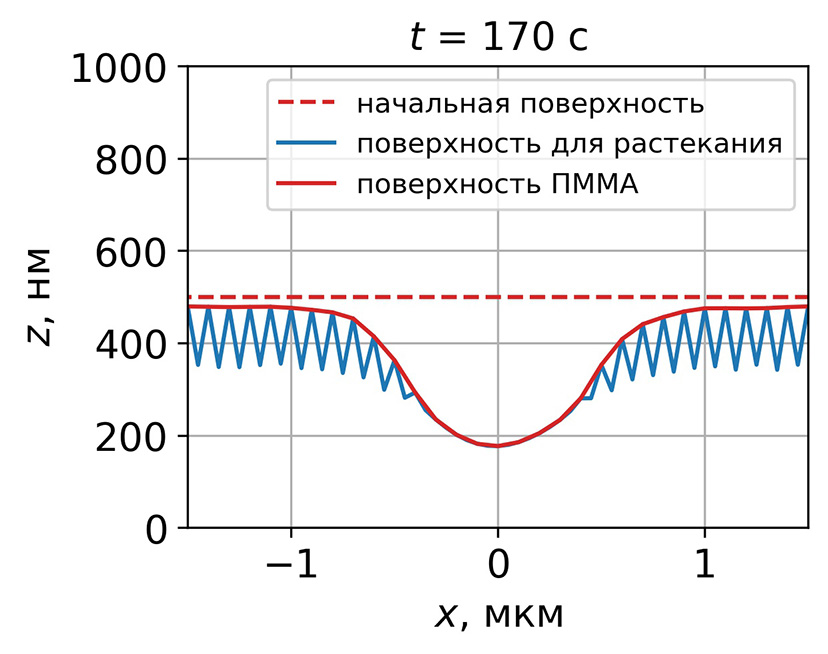
\includegraphics[width=\linewidth]{DEBER_example/example_170_200} \\
		\includegraphics[width=\linewidth]{DEBER_example/example_370_NEW_2} \\
		\vspace{-13em} \\ \text{\hspace{-0.1em} г}) \\ \vspace{13em}
	\end{minipage}
	\vspace{-3em}
	\caption{
		Процесс моделирования профиля, получаемого методом СЭЛТР.
		Условия экспонирования: $E$ = 20 кэВ, $T$ = 150 $^{\circ}$C/c, $t_\mathrm{exp}$ = 100 с, плотность тока экспонирования на единицу длины $j_\mathrm{l}$ = 10 пА/см.
		Скорость охлаждения образца составляла 1~$^{\circ}$C/с.
		Красная пунктирная линия обозначает начальное положение поверхности слоя ПММА, черные точки -- координаты точек входа электронного пучка в слой ПММА (показана каждая 30-я точка).}
	\label{fig:DEBER_example}
\end{figure}

На основе разработанной модели можно сделать общие заключения о процессе формирования линии в методе СЭЛТР.
На начальной стадии СЭЛТР экспонирование образца вызывает деполимеризацию резиста и формирование в нем микрополостей, однако, процессы растекания еще не проявляются заметным образом за счет относительно высокого значения вязкости резиста (рисунок~\ref{fig:DEBER_example}a).
В дальнейшем среднечисловая молекулярная масса и, соответственно, вязкость резиста снижаются до значений, при которых растекание резиста становится явно выраженным, что активирует процесс заполнения микрополостей (рисунки~\ref{fig:DEBER_example}б, \ref{fig:DEBER_example}в).
С этого момента времени процессы деполимеризации резиста, образования новых и заполнения старых микрополостей начинают протекать одновременно на фоне непрерывного уменьшения вязкости резиста.
При окончании экспонирования прекращается образование новых микрополостей и уменьшение вязкости резиста, и дальнейшее охлаждение образца сопровождается только заполнением существующих микрополостей (рисунок~\ref{fig:DEBER_example}г).
